\documentclass[compress]{beamer}
\usepackage{setspace}
\usepackage{multicol}
\mode<presentation>
{
  %\usetheme{Warsaw}
  %\usecolortheme{spruce}
  % or ...
	%\useoutertheme{infolines}
  %\setbeamercovered{transparent}
  
  \usetheme{CambridgeUS}
    \setbeamercolor{item projected}{bg=darkred}
    \setbeamertemplate{enumerate items}[default]
    \setbeamertemplate{navigation symbols}{}
    \setbeamercovered{invisible}
    \setbeamercolor{block title}{fg=darkred}
    \setbeamercolor{local structure}{fg=darkred}
  
  % or whatever (possibly just delete it)
}

\usepackage{verbatim} 
\usepackage{listings}
\usepackage{tikz}

%\usepackage[noend]{algpseudocode}
\usepackage{algorithm,algorithmic}


\usepackage{amsmath}
\usepackage{blindtext}
\usepackage{wrapfig}
\usepackage{amsfonts}
\usepackage{graphicx}
\usepackage{multirow}
\usepackage{caption}
\usepackage{subcaption}
\usepackage{enumerate}
\usepackage[colorinlistoftodos]{todonotes}


\usetikzlibrary{arrows}
\usetikzlibrary{shapes}
\tikzstyle{block}=[draw opacity=0.7,line width=1.4cm]

\newcommand{\bigpause}{\bigskip \pause}
\newcommand\azul[1]{{\color{blue}#1}}
\lstloadlanguages{C++}
\lstnewenvironment{code}
	{%\lstset{	numbers=none, frame=lines, basicstyle=\small\ttfamily, }%
	 \csname lst@SetFirstLabel\endcsname}
	{\csname lst@SaveFirstLabel\endcsname}
\lstset{% general command to set parameter(s)
	language=C++, basicstyle=\footnotesize\sffamily, keywordstyle=\slshape,
	emph=[1]{tipo,usa}, emphstyle={[1]\sffamily\bfseries},
	basewidth={0.47em,0.40em},
	columns=fixed, fontadjust, resetmargins, xrightmargin=5pt, xleftmargin=15pt,
	flexiblecolumns=false, tabsize=2, breaklines,	breakatwhitespace=false, extendedchars=true,
	numbers=left, numberstyle=\tiny, stepnumber=1, numbersep=9pt,
	frame=l, framesep=3pt,
}

\usepackage[spanish]{babel}
% or whatever

\usepackage[utf8]{inputenc}

\usepackage{graphicx}
\usepackage{caption}
\usepackage{multirow}
\usepackage{subcaption}
\usepackage{wrapfig}

\usepackage{times}
\usepackage[T1]{fontenc}
% Or whatever. Note that the encoding and the font should match. If T1
% does not look nice, try deleting the line with the fontenc.

\DeclareMathOperator*{\argmax}{arg\,max}
\DeclareMathOperator*{\avg}{avg}
\DeclareMathOperator*{\stdev}{stdev}
\newcommand\normtwo[1]{\left\lVert#1\right\rVert_2}


\title[Defensa de tesis de licenciatura] % (optional, use only with long paper titles)
{Análisis y predicción de la búsqueda visual humana}

\author[Melanie Sclar] % (optional, use only with lots of authors)
{~Melanie Sclar}
% - Give the names in the same order as the appear in the paper.
% - Use the \inst{?} command only if the authors have different
%   affiliation.
\institute[UBA] % (optional, but mostly needed)
{
  %\inst{1}%
  Facultad de Ciencias Exactas y Naturales\\
  Universidad de Buenos Aires
}
%\date[PAP] % (optional, should be abbreviation of conference name)
%{Problemas, Algoritmos y Programación}

% Delete this, if you do not want the table of contents to pop up at
% the beginning of each subsection:
\AtBeginSubsection[]
{
  \begin{frame}<beamer>{Contenidos}
    \tableofcontents[currentsection,currentsubsection]
  \end{frame}
}

%\newcommand{\be}{\begin{equation*}}
\newcommand{\ee}{\end{equation*}}
\newcommand{\state}[1]{\left|\,#1\,\right\rangle}
\newcommand{\costate}[1]{\left\langle\,#1\,\right|}
\newcommand{\trace}{\text{Tr}}
\newcommand{\su}{\uparrow}
\newcommand{\sd}{\downarrow}
\newcommand{\im}{\text{Im}}
\newcommand{\re}{\text{Re}}

% If you wish to uncover everything in a step-wise fashion, uncomment
% the following command:

%\beamerdefaultoverlayspecification{<+->}


\begin{document}
\pgfdeclarelayer{background}
\pgfsetlayers{background,main}
\begin{frame}
  \titlepage
\end{frame}


\section{Introducción}
\begin{frame}{Motivación}
\begin{itemize}
\item Uno de los desafíos centrales de la ciencia cognitiva y de la neurociencia de la visión es entender cómo percibimos una escena visual.
\item Más de medio siglo después de las primeras experimentaciones, todavía no existe una teoría formal de la interacción entre la percepción y los movimientos oculares.
\item Una idea que se viene fortaleciendo en la última década es la aplicación de un marco bayesiano para explicar cómo el cerebro es capaz de generalizar y realizar inferencias sobre entornos ruidosos y saturados de información.
\item \textbf{Buscamos dar un paso adelante en el entendimiento de la visión humana combinando modelos para comprenderla a nivel algorítmico.}
\end{itemize}
\end{frame}

\begin{frame}{Agudeza visual}
\begin{itemize}
\item Podemos ver en detalle solo una pequeña porción del campo visual, aquella que cae en un área de la retina llamada \textit{fóvea}.
\item Debido a las limitaciones de agudeza en la retina, los movimientos oculares son necesarios para procesar detalles.
\end{itemize}
\end{frame}

\begin{frame}{Movimientos oculares}
\begin{itemize}
\item Existen dos categorías básicas de movimientos oculares: las sacadas y las persecuciones suaves.
\item Los ojos rotan rápidamente para fijar la vista en una nueva posición y centrar la fóvea. Este proceso ocurre varias veces por segundo sin involucrar la consciencia de las personas.
\end{itemize}
\end{frame}

\begin{frame}
\begin{center}
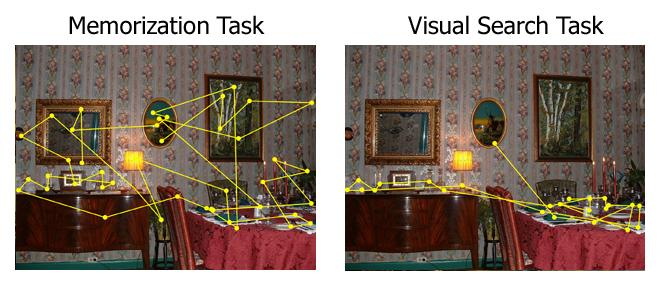
\includegraphics[width=0.8\textwidth]{images/castelhano-fixations.jpg}
\end{center}

Las ubicaciones de las fijaciones no son aleatorias y los patrones que describen dependen fuertemente de la tarea que realice. Aún si no damos ninguna tarea en particular, las personas miran en puntos que les resultan más informativos.
\end{frame}

\begin{frame}{Modelos de saliencia}

\begin{itemize}
\item Como no podemos procesar toda la información de una imagen a la vez, restringimos los procesos complejos a un área reducida que es considerada interesante. 
\item Después, analizamos distintas regiones una atrás de la otra. 
\item ¿Cómo decidimos qué región seleccionar para captar nuestra atención primero?
\item Este es el problema de decidir qué regiones son más salientes, y desde la computación se crean \textbf{mapas de saliencia} que predicen estas regiones.
\end{itemize}

\end{frame}

\begin{frame}{Modelos de saliencia (2)}
\begin{center}
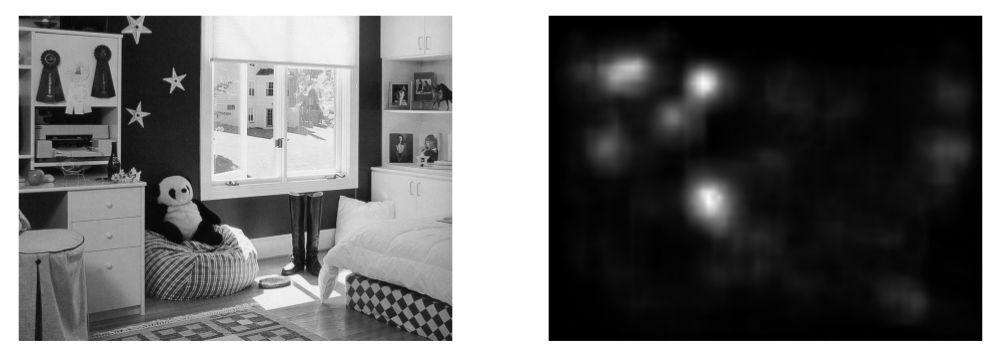
\includegraphics[width=0.9\textwidth]{images/ejemplo-mlnet.png}
\end{center}

{\small Los mapas de saliencia aún no logran reproducir a la perfección los lugares de la imagen que más llaman la atención humana, pero año a año hay avances en este área.\\}

\bigskip

{\small En \texttt{http://saliency.mit.edu/} hay una recopilación de los mejores modelos a la fecha. De ahí, tomamos tres: Judd, SAM y MLNet.}

\end{frame}

\begin{frame}{Modelos de saliencia (3)}
\begin{itemize}
\item Los modelos de saliencia toman en cuenta diferentes factores que afectan la atención visual, como ser los colores, el contraste, la orientación, la presencia de texto o humanos, entre otros.
\item Estos factores se clasifican en dos categorías: \textit{bottom-up} (dependiendo únicamente de las características de la imagen) y \textit{top-down} (dependiendo de la tarea que se realice).
\end{itemize}
\end{frame}

\begin{frame}{Búsqueda visual}
% definir búsqueda visual?
En la búsqueda visual se combinan factores \textit{top-down} y \textit{bottom-up}, de tal forma que a veces regiones muy salientes se ignoran porque son poco relevantes para la tarea.

\bigskip
La saliencia suele funcionar mejor en escenas artificiales que en naturales, porque en estos últimos afectan también factores contextuales y semánticos.

\bigskip

Esto no significa que la saliencia deje de ser relevante, pero se suele combinar ésta con mapas más específicos como detectores de target o un mapa de apariencia esperada del target.

\end{frame}

% pasar para más adelante
%\begin{frame}{Modelos de movimientos oculares en imágenes}
%\end{frame}

\begin{frame}{Métricas de comparación de \textit{scanpaths}}
No hay consenso sobre qué métrica utilizar para comparar scanpaths, ya que hay muchos factores a tener en cuenta. Así, algunos de los más famosos son:
\begin{itemize}
\item Cantidad de fijaciones hasta encontrar el target
\item Edit distance de strings, con variaciones según las operaciones que se permitan: inserción, eliminación o sustitución de un caracter.
% edit distance lo explico con un ejemplo en el pizarrón 
\item Ángulos entre fijaciones
\item Distancia de Mannan
\end{itemize}
\end{frame}

\begin{frame}{Métricas de comparación de \textit{scanpaths}}
{Edit distance - ejemplo}

\begin{center}
    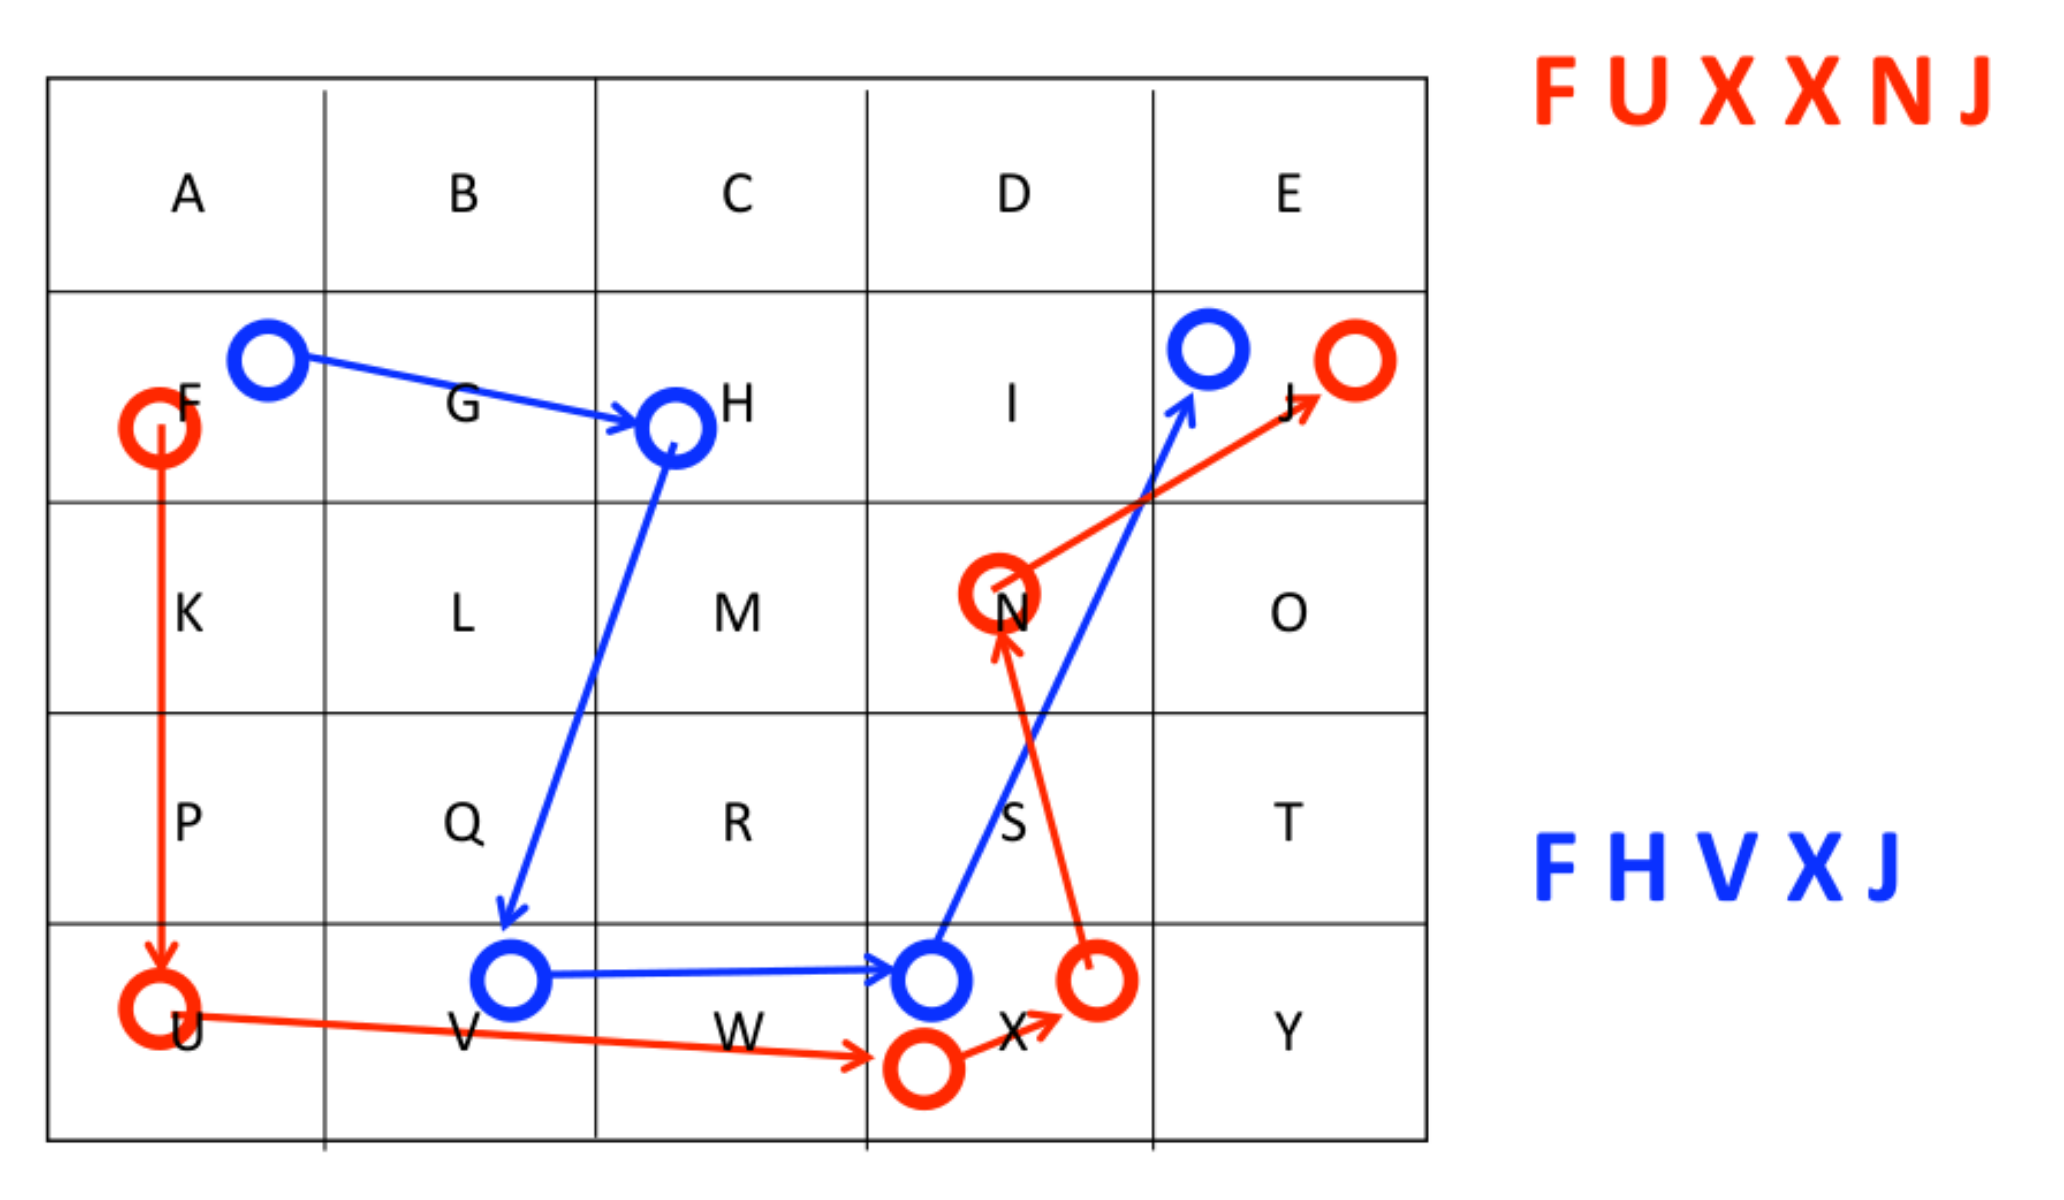
\includegraphics[width=\linewidth]{images/edit-distance.png} 
\end{center}

\end{frame}


\section{Experimentos}
\subsection{Creación de un corpus de imágenes}
\begin{frame}{Creación de un corpus de imágenes de interiores}
\begin{itemize}
\item Recolectamos 134 imágenes de interiores de $768 \times 1024$ píxeles.
\item Las imágenes son en blanco y negro y no tienen personas ni texto.
\item Recortamos varios targets por imagen de diferentes y seleccionamos al azar uno por imagen, siempre y cuando fuera menor a $72 \times 72$.
\item Luego uniformizamos los targets para que todos tengan $72 \times 72$ píxeles.
\end{itemize}
\end{frame}

\subsection{Experimento de búsqueda visual}
\begin{frame}{Diseño del experimento de búsqueda visual}

\begin{itemize}
\item Utilizamos un Eye Tracker para grabar los movimientos oculares del ojo derecho. Los participantes solo pueden mover la vista y no la cabeza durante el experimento.
\item Realizamos 134 ensayos, uno por imagen, en tres bloques. Entre cada bloque el participante descansa y se recalibra el Eye Tracker.
\item Al comienzo de cada ensayo se checkea que siga recalibrado con el \textit{drift correction}.
\end{itemize}

\end{frame}

\begin{frame}
\begin{figure}[!b]
    \centering
    \begin{subfigure}[b]{0.32\textwidth}
        \centering
        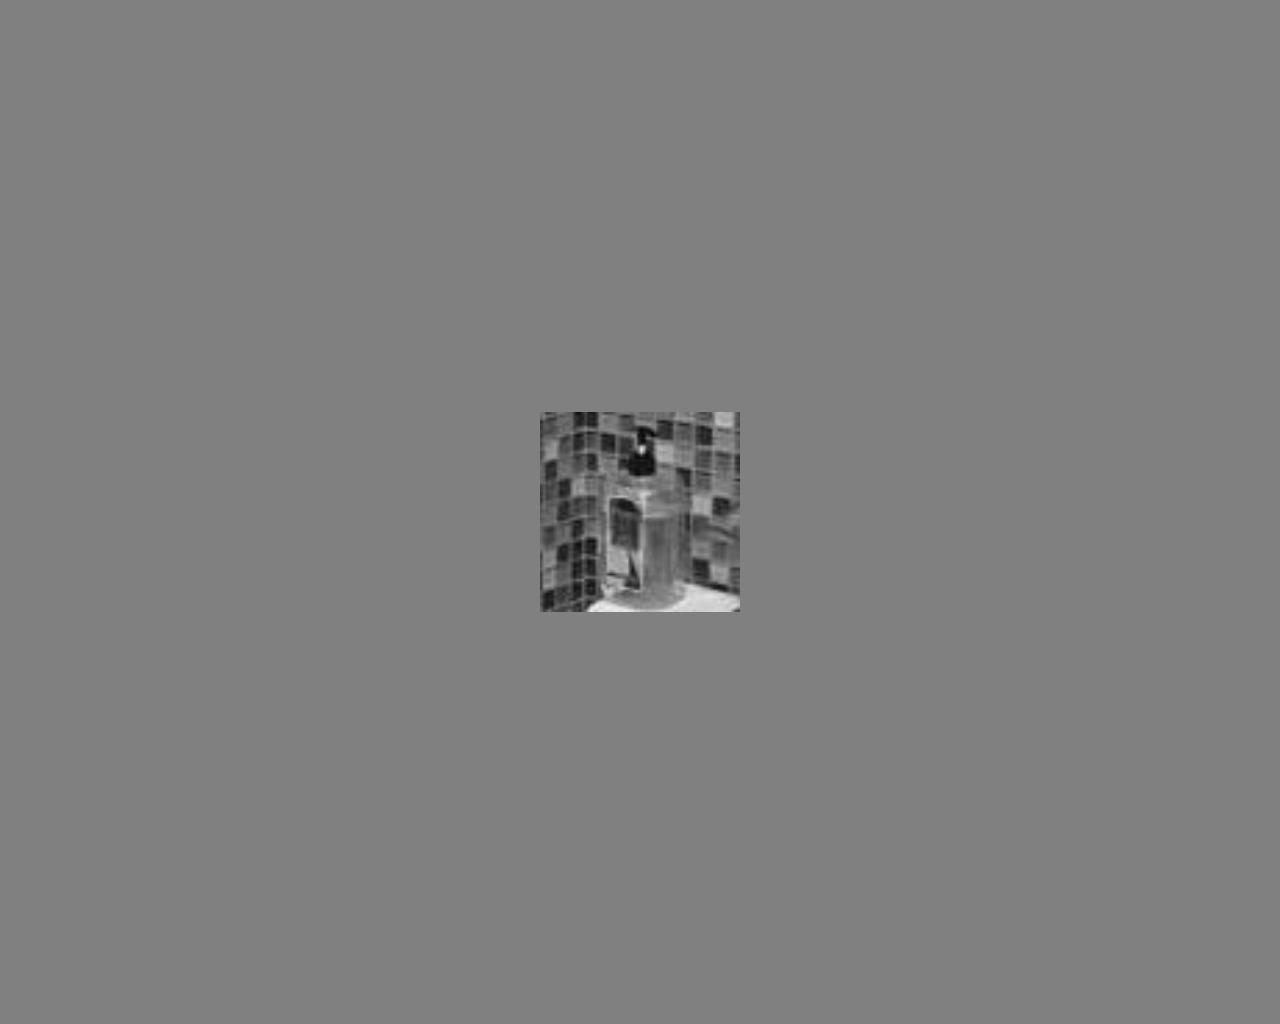
\includegraphics[width=\linewidth]{images/target_bathroom.jpg} 
        \caption{Muestra de target} \label{fig:expe-etapa-1}
    \end{subfigure}
    \hfill
    \begin{subfigure}[b]{0.32\textwidth}
        \centering
        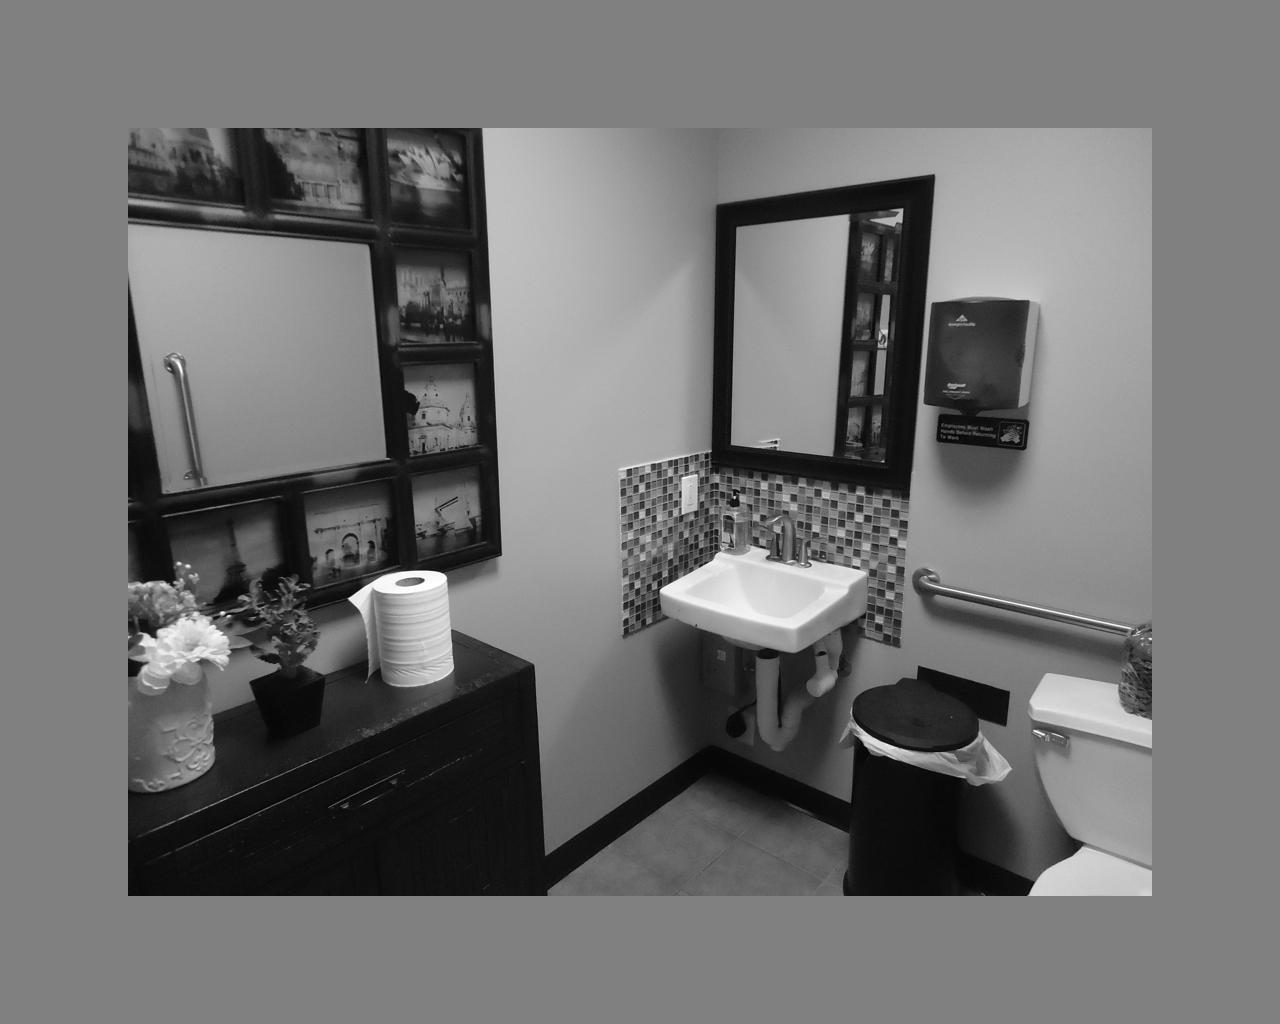
\includegraphics[width=\linewidth]{images/full_bathroom.jpg} 
        \caption{Imagen completa} \label{fig:expe-etapa-3}
    \end{subfigure}
    \hfill
    \begin{subfigure}[b]{0.32\textwidth}
        \centering
        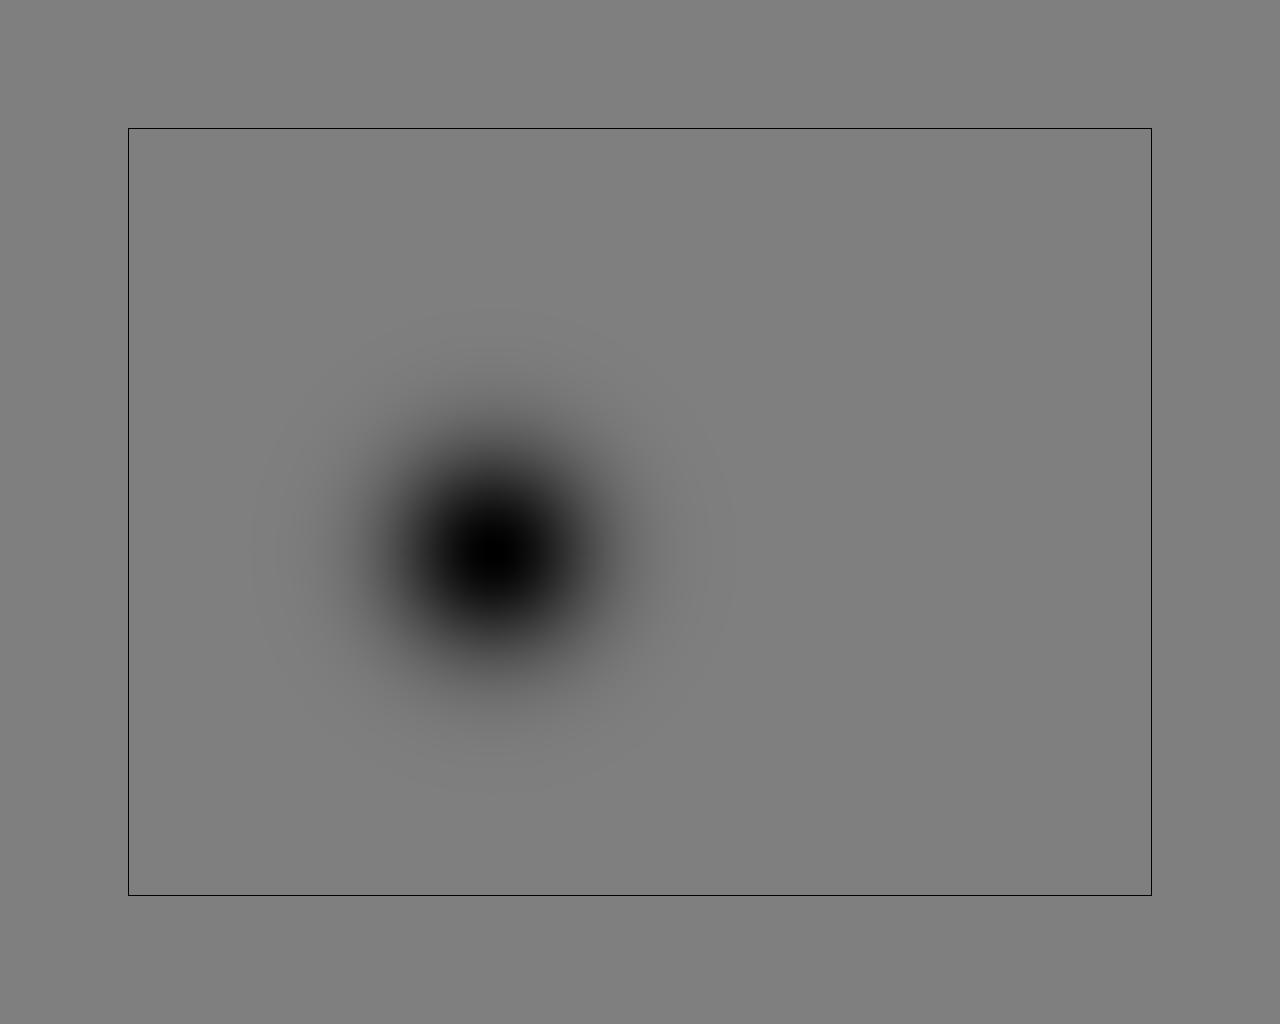
\includegraphics[width=\linewidth]{images/subjective_response_ahora.jpg} 
        \caption{Respuesta subjetiva} \label{fig:expe-etapa-4}
    \end{subfigure}
\end{figure}

Se fuerza a los sujetos a mirar en un punto negro a 300 píxeles del target. Este lugar varía por imagen pero es el mismo para todos los sujetos.

\end{frame}

\begin{frame}
\begin{itemize}
\item Según el ensayo elegimos aleatoriamente la cantidad de sacadas que se le permite realizar a las personas antes de cortar el ensayo y pedirle el reporte subjetivo. 
\item Elegir la distribución de cantidad de fijaciones no fue fácil, pues quisimos maximizar la cantidad de ensayos con varias fijaciones donde los sujetos no hayan encontrado el target.
\end{itemize}

\bigskip

\begin{table}[h]
\centering
\tiny
\begin{tabular}{c|c|c|c|c|c|c|c|c|c|}
\cline{2-10}
                                           & \multirow{2}{*}{\textbf{\tiny \begin{tabular}[c]{@{}c@{}} Cantidad \\ de sujetos\end{tabular}}} & \multirow{2}{*}{\textbf{\tiny \begin{tabular}[c]{@{}c@{}} Cantidad \\ de imágenes \end{tabular}}} & \multicolumn{7}{c|}{\textbf{Cantidad de sacadas}}                                        \\ \cline{4-10} 
                                           &                                                                                          &                                                                                                      & \textbf{2} & \textbf{3} & \textbf{4} & \textbf{8} & \textbf{12} & \textbf{16} & \textbf{64} \\ \hline
\multicolumn{1}{|c|}{\textbf{Tarea 1}}     & 3                                                                                        & 108                                                                                                  & 20,4\%    &            & 20,4\%    & 20,4\%    &             & 20,4\%     & 18,4\%     \\ \hline
\multicolumn{1}{|c|}{\textbf{Tarea 2}}     & 2                                                                                        & 108                                                                                                  & 25\%       &            & 25\%       & 25\%       &             & 12,5\%     & 12,5\%     \\ \hline
\multicolumn{1}{|c|}{\textbf{Tarea 3}}     & 6                                                                                        & 108                                                                                                  & 25\%       & 25\%       & 25\%       & 25\%       &             &             &             \\ \hline
\multicolumn{1}{|c|}{\textbf{Tarea final}} & 17                                                                                       & 134                                                                                                  & 13,4\%    &            & 14,9\%    & 29,9\%    & 41,8\%     &             &             \\ \hline
\end{tabular}
\caption{\label{tab:tareas} Distribuciones de cantidad de sacadas utilizadas en la puesta a punto del experimento.}
\end{table}


\end{frame}


\begin{frame}
\begin{itemize}
\item Tomamos datos de 30 participantes, pero 2 no pudieron ser grabados adecuadamente por un error del software.
\item De los 28 sujetos que obtuvimos, 3 fueron mujeres y 25 varones, todos ellos estudiantes o docentes de la FCEyN - UBA.
\end{itemize}

\bigskip
\bigskip

Como los target son de diferentes clases de objetos, notamos que para diseñar buenos algoritmos necesitábamos entender semánticamente a qué clase de objeto pertenece cada una. Para esto realizamos otro experimento.
\end{frame}

\subsection{Experimento de detección de objetos}
\begin{frame}{Experimento de detección de objetos}
\begin{itemize}
\item Mostramos cada uno de los target durante 3 segundos y luego le pedimos a los participantes que digan qué objeto es el de la imagen de tres formas distintas.
\item Los target se muestran en orden aleatorio, y son los mismos del experimento original.
\item Si el usuario no reconoce el objeto, existe una opción a ese fin.
\item Esta tarea se puede realizar online en varios días. Si quieren participar, sigue abierta en \texttt{http://objetos.gpoesia.com}
\item Obtuvimos datos de 17 participantes. No todos terminaron el experimento, pero tuvimos en promedio 10.5 respuestas por imagen.
\end{itemize}
\end{frame}

\section{Análisis del comportamiento}

\begin{frame}
En algunos ensayos la mirada se posó tan cerca del target (a menos de $1.25^{\circ}$ del centro) que llegó a fijar parte del mismo con la visión foveal. Por eso consideramos para nuestros análisis que el target en realidad fue encontrado aunque la vista no haya sido posada sobre el target.

\bigskip

Analizamos diferentes aspectos del experimento que utilizaremos más adelante, y mencionamos rápidamente.
\end{frame}


\begin{frame}{Longitud de las sacadas}
\begin{center}
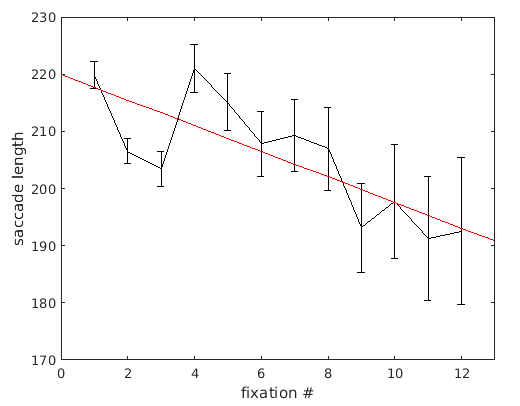
\includegraphics[width=0.6\textwidth]{images/mean-sacclen.png}
\end{center}

Vemos que la longitud de las sacadas decrece a lo largo del tiempo, consistentemente con otros trabajos.
\end{frame}

\begin{frame}{Sesgo de la fijación central}
\begin{center}
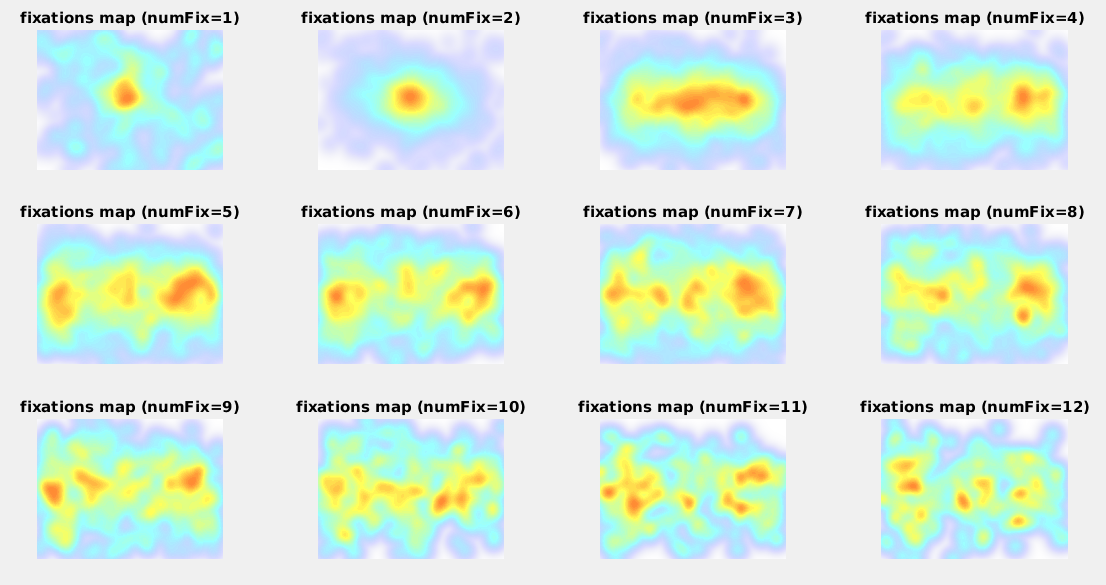
\includegraphics[width=0.9\textwidth]{images/heatmap-per-fix.png}
\end{center}

Notar que el sesgo también se marca en la primera fijación. \end{frame}

%\begin{frame}

%\begin{center}
%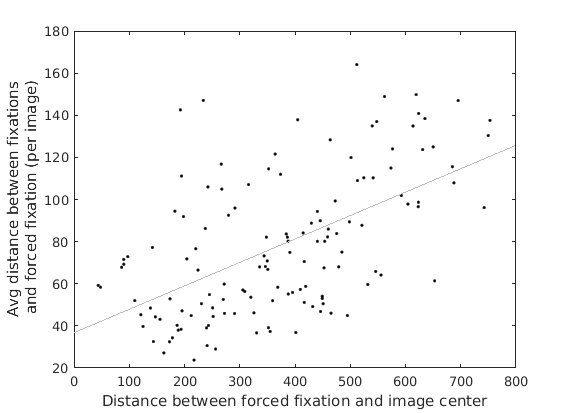
\includegraphics[width=0.6\textwidth]{images/scatter-first-fixation.png}
%\end{center}

%{\scriptsize
%Notar que el sesgo también se marca en la primera fijación. Algunos sujetos movieron rápidamente los ojos desde la fijación pedida hacia el centro, y grabamos la primera fijación allí.}

%\bigskip

%{\scriptsize Se observa que la distancia del punto de la primera fijación al centro de la imagen correlaciona con cuán bien los participantes respetan la instrucción de mantener la mirada en el punto pedido.}
%\end{frame}

\begin{frame}{Cambios en incerteza según cantidad de fijaciones}
\centering
  \begin{columns}[T]
    \begin{column}{.4\textwidth}

        {\scriptsize

        Vemos que los radios de los círculos son muy diferentes según si el target fue encontrado o no. Esto muestra que los sujetos tienen consciencia de que encontraron el target. \\ \bigskip

        Además vimos en la tesis que existe un efecto "desmoralizador": si llevamos algunos ensayos sin encontrar el target, la probabilidad de colocar un círculo más grande se incrementa. Lo mismo vale pero en mucha menor medida para el caso opuesto (varios ensayos encontrando targets). \par}


    \end{column}
    \begin{column}{.6\textwidth}
        \begin{center}
        \centering
        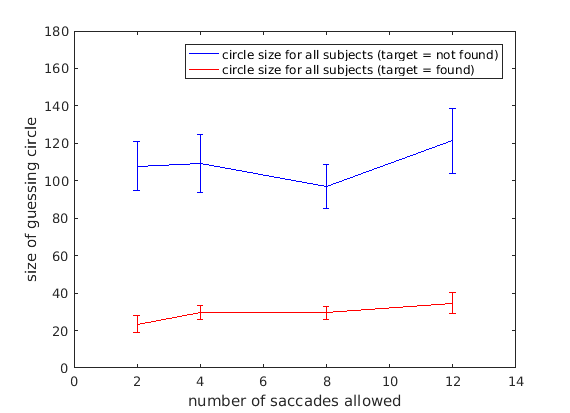
\includegraphics[width=\linewidth]{images/mean_circle_size.png}
        \end{center}
    \end{column}
  \end{columns}
\end{frame}

% esto se puede saltear
%\begin{frame}{Influencia de ensayos anteriores en la respuesta actual}
%\begin{center}
%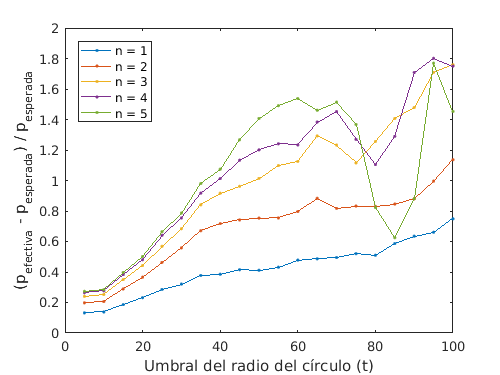
\includegraphics[width=0.6\textwidth]{images/desconfianza-rta-dif-relativa.png}
%\end{center}
%\end{frame}

\begin{frame}
Ahora mostraremos los distintos modelos predictivos que proponemos. Estos modelos se dividen en dos clases según si predicen las regiones a ser fijadas (\textbf{modelos estáticos}) o si predicen el orden de las fijaciones (\textbf{modelos dinámicos}).
\end{frame}

\section{Modelos estáticos}

\begin{frame}
Crearemos nuestros propios modelos estáticos, basados en el mapa de saliencia creado por Judd. Lo compararemos con dos modelos del estado del arte, SAM y MLNet. 

\medskip
Si bien los mapas de saliencia no son predictores perfectos en tareas de búsqueda visual son buenos orientadores de la atención visual.

\bigskip
\bigskip
Antes de referirnos a cómo creamos los modelos tenemos que entender cómo vamos a medir su performance.
\end{frame}


\begin{frame}{Medidas de performance}

\begin{itemize}
{\small 
\item Tomamos los mapas de saliencia como un clasificador binario de los píxeles. Un porcentaje dado de los píxeles de una imagen se clasifican como positivos y el resto negativos.
\item Se grafica para varios porcentajes el True Positive Rate (TPR), que indica qué porción de las fijaciones caen en la región saliente.
}
\end{itemize}

\begin{figure}[b]
    \centering
    \begin{subfigure}[t]{0.3\textwidth}
        \centering
        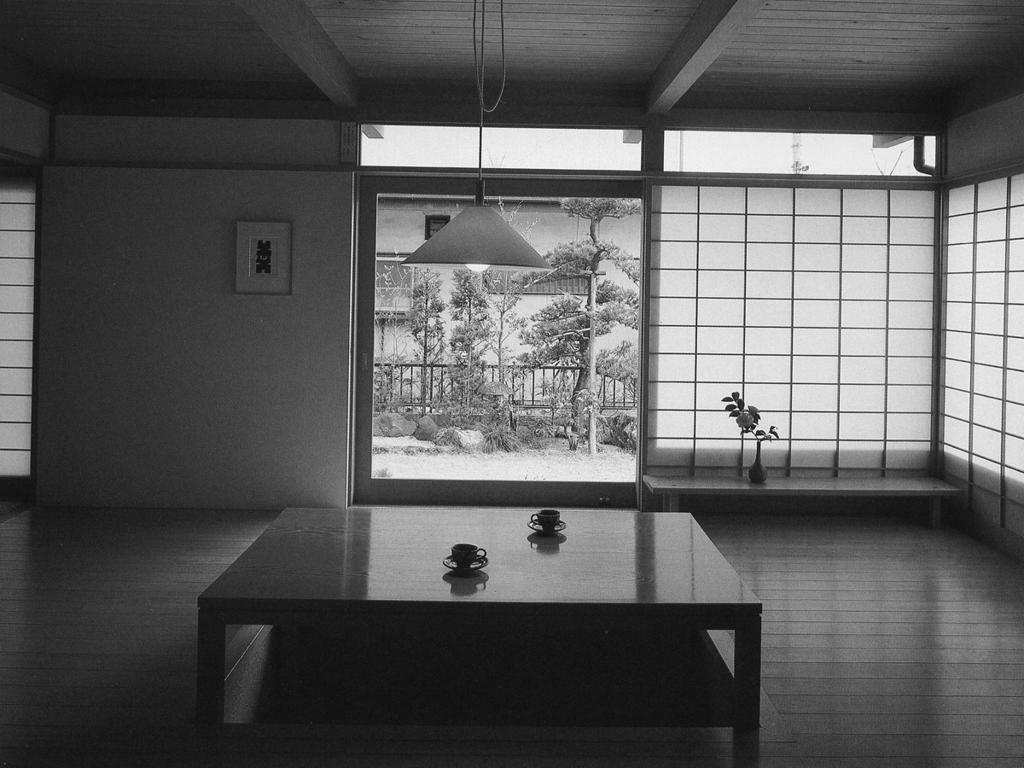
\includegraphics[width=\linewidth]{images/grayscale_100_oliva.jpg}
        \caption{\footnotesize Imagen original} \label{fig:grayscale_100_oliva}
    \end{subfigure}
    \hfill
    \begin{subfigure}[t]{0.3\textwidth}
        \centering
        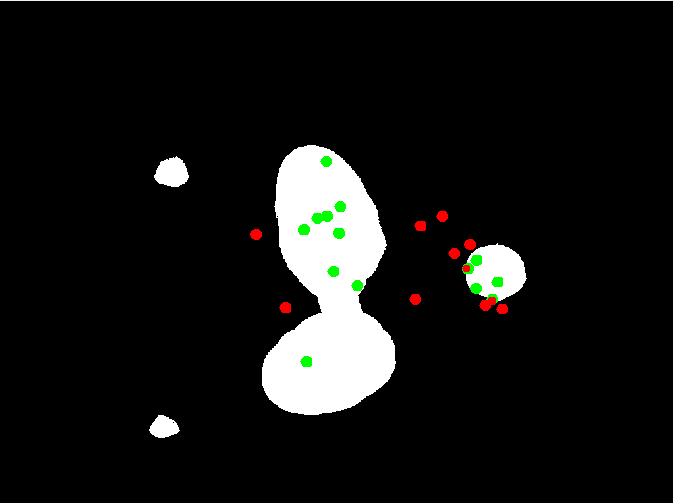
\includegraphics[width=\linewidth]{images/example-salient-percent-8-14.png} 
        \caption{\footnotesize 8.14\% más saliente de la imagen según SAM} \label{fig:example-salient-percent-8-14}
    \end{subfigure}
	\hfill
	\begin{subfigure}[t]{0.3\textwidth}
        \centering
        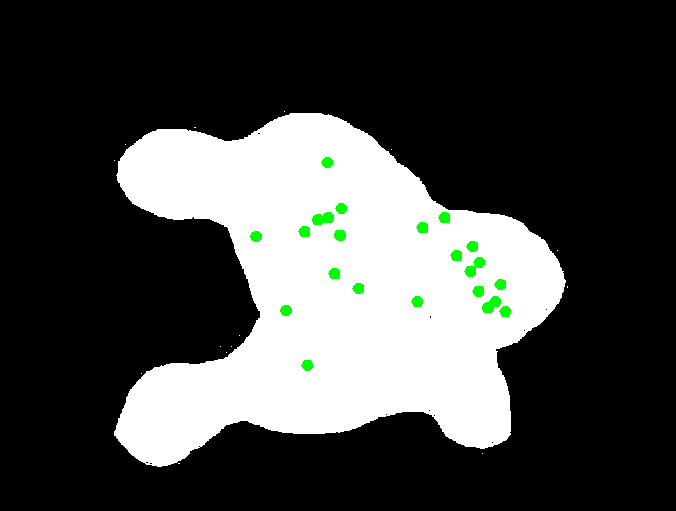
\includegraphics[width=\linewidth]{images/example-salient-percent-27-73.png} 
        \caption{\footnotesize
27.73\% más saliente de la imagen según SAM} \label{fig:example-salient-percent-27-73}
    \end{subfigure}
\end{figure}

\end{frame}

\begin{frame}{Modelos de saliencia como predictores de fijaciones}

\begin{figure}
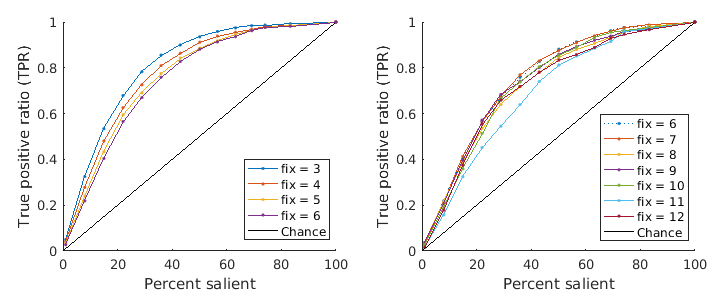
\includegraphics[width=\linewidth]{images/sam_all_fix_small.png} 
\caption{Performance de SAM}
\end{figure}

{\footnotesize Tanto SAM como MLNet predicen mejor las primeras fijaciones que las últimas. Mostamos aquí solo SAM. Veamos cómo es el modelo de Judd y como lo extenderemos para mejorar la performance recién mostrada.}

\end{frame}

\begin{frame}{Modelo de saliencia de Judd}
\begin{itemize}
\item Se realiza un mapa de saliencia por imagen tomando las fijaciones de los humanos y suavizándolas con un filtro gaussiano. Este mapa es tomado como \textit{ground truth} para entrenar su modelo.
\item Para entrenar su modelo Judd toma 10 píxeles al azar del 20\% más saliente del mapa de saliencia  \textit{ground truth} y los identifica como píxeles salientes. Asimismo, toma 10 píxeles al azar del 30\% menos saliente y los toma como píxeles negativos.
\end{itemize}
\end{frame}

\begin{frame}{Modelo de saliencia de Judd (2)}
\begin{itemize}
\item Computa 33 features por imagen, que incluyen: mapas de colores (RGB), mapa de intensidad, mapa de orientación, mapa de contraste, mapa de distancia al centro de la imagen, mapa de distancia al horizonte, mapas de detección de rostros, autos, personas y dos mapas de saliencia base.
\item Separamos las imágenes en dos conjuntos: uno de entrenamiento y uno de testing. 
\item Luego entrena una Support Vector Machine (SVM) con las muestras positivas y negativas del conjunto de imágenes de entrenamiento. Utiliza un kernel lineal por su simplicidad, y porque probó otros kernels pero no mejoró la performance.
\item \textbf{Este modelo permite muy fácilmente agregar y remover features} que se adapten mejor a nuestra tarea.
\end{itemize}
\end{frame}

\begin{frame}
\begin{itemize}
\item Tomaremos el modelo de Judd y lo adaptaremos a nuestra tarea, que es de búsqueda visual.
\item Tomamos 100 imágenes para el conjunto de entrenamiento y 34 imágenes para el conjunto de testing.
\item Removemos los features de rostros, autos, personas y los features de colores pues no aparecen en nuestra tarea.
\item Utilizamos SAM y MLNet como mapas de saliencia base, que son del estado del arte.
\bigskip
\item Extendemos Judd con dos tipos de mapas que extraen información del target:
\begin{enumerate}[I.]
\item Mapas teniendo en cuenta el aspecto netamente visual del target
\item Mapas teniendo en cuenta la semántica de la imagen mostrada. Esto incluye el reconocimiento de la clase de objeto a la que pertenece el target y la unión de este conocimiento con el de las experiencias previas del sujeto.
\end{enumerate}
\end{itemize}
\end{frame}

\begin{frame}{Extensión de Judd - tipo I}

\begin{itemize}
\item El primer mapa es del de la \textit{cross correlation} del target y la imagen original.
\item El segundo mapa intenta representar una \textbf{similitud de bajo nivel} entre el target y una porción de la imagen.
\end{itemize}

\begin{figure}
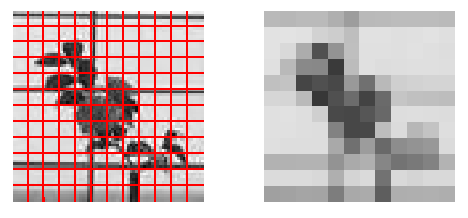
\includegraphics[width=0.7\linewidth]{images/grilla-gorda.png} 
\end{figure}

\end{frame}

\begin{frame}{Extensión de Judd - tipo II}

  \begin{columns}[T]
    \begin{column}{.65\textwidth}
        \begin{itemize}
        \item Queremos crear un mapa teniendo en cuenta la semántica de la imagen mostrada.
        \item Recordemos que sabemos a qué clase de objeto pertenece cada target por nuestro experimento online. 
        \item Además, encontramos un dataset llamado LabelMe que posee 8000 imágenes segmentadas y parcialmente anotadas por la comunidad.
        \end{itemize}
    \end{column}
    \begin{column}{.35\textwidth}
        \begin{figure}
        \begin{center}
        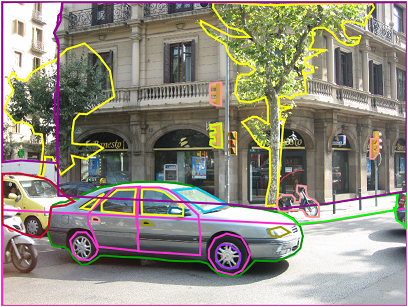
\includegraphics[width=\textwidth]{images/label-me-example.png} 
        \end{center}
        \end{figure}
    \end{column}
  \end{columns}

\end{frame}

\begin{frame}{Outline del mapa de tipo II}
\begin{itemize}
\item Detectamos a qué clase de objeto pertenece cada target con una palabra en español con nuestra tarea online.
\item Medimos la distancia de la palabra que representa a cada target respecto de algunas palabras que denotan posición en una escena de interiores (por ejemplo, mesa, piso, techo, ventana, pared
- las llamaremos \textbf{palabras posicionales}). 
\item Se toma la palabra posicional más cercana y ésta representará la posición probable del target: esto hipotetizamos que será un indicio de los sectores de la imagen asociados a la palabra posicional. 
\item El mapa de features será entonces el mapa de las regiones más fuertemente asociadas a la palabra posicional.
\end{itemize}
\end{frame}

\begin{frame}
\begin{figure}
\begin{center}
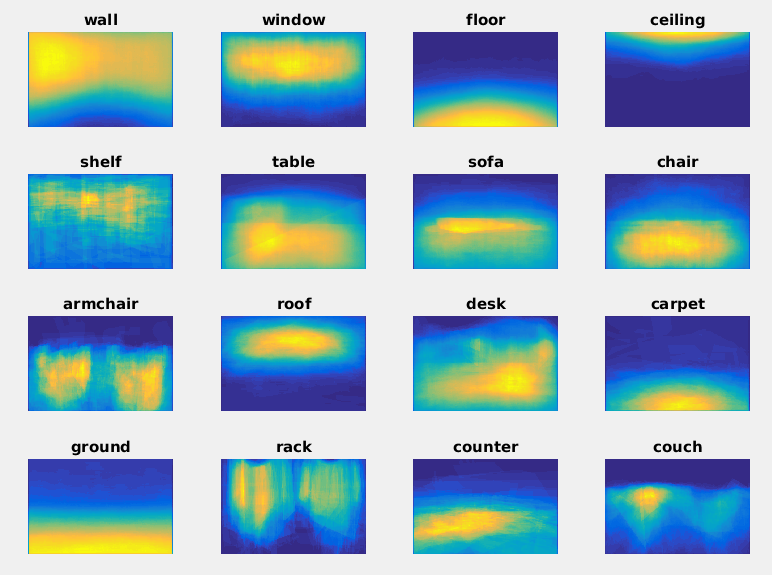
\includegraphics[width=0.75\textwidth]{images/labelme-global-features-without-horizon.png} 
\end{center}
\end{figure}

{\small Creamos un mapa posicional por cada una de las 16 palabras posicionales elegidas, superponiendo las regiones anotadas con la palabra en LabelMe.}
\end{frame}
% hago dibujo en el pizarrón de taza ===> vector de taza, mesa ==> vector de mesa 

%\begin{frame}
%Hay muchos puntos donde se puede seguir explorando en este mapa de features, como tener en cuenta la línea del horizonte para uniformizar las imágenes. 

%Existen detectores del horizonte, pero fueron entrenados en imágenes de exteriores, que tienen un comportamiento distinto que las de interiores. 

%Como trabajo futuro
%\end{frame}

\subsection{Resultados de modelos estáticos}
\begin{frame}
\begin{itemize}
\item Ya comentamos que medimos la performance mirando el TPR vs. el porcentaje que es considerado saliente
\item En este tipo de tareas se suele tomar a los humanos como \textit{baseline}. Hemos visto que los humanos son fuertemente consistentes en las primeras fijaciones, y el nivel de predicción baja con el número de fijaciones.
\end{itemize}

\bigskip
Veamos cómo el modelo de Judd extendido con nuestras features predice las fijaciones humanas, separando las fijaciones en 3 grupos: tercera fijación, fijaciones 4 a 6 y fijaciones 7 a 12.

\end{frame}

\begin{frame}{Resultados tercera fijación}
\begin{center}
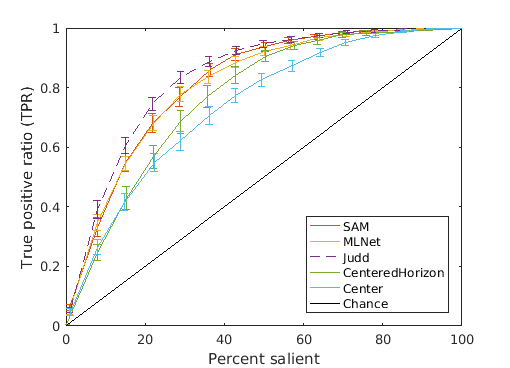
\includegraphics[width=0.6\textwidth]{images/results_fix_3_to_3_all.png} 
\end{center}

{\footnotesize En este gráfico no se separan los sujetos en conjunto de entrenamiento y conjunto de testing. }
\end{frame}

\begin{frame}
\begin{itemize}
\item También hicimos experimentaciones separando los sujetos en un conjunto de entrenamiento y otro de test (25\% para el test set, 75\% para el training set), donde se ve que la performance es muy similar a la alcanzada por los humanos.
\item Como esto nos deja con muy pocos datos para el test set (a lo sumo $7 \times 34$) los resultados no son concluyentes.
\item Además, no pudimos concluir cuáles de los 3 features que agregamos son los que tienen más peso, pues depende del conjunto de entrenamiento elegido.
\end{itemize}
\end{frame}

\begin{frame}

La tercera fijación es especialmente importante pues es la que utilizamos como mapa de base para los modelos dinámicos.

\bigskip

Utilizamos la tercera fijación pues las dos anteriores están afectadas por el sesgo de la fijación pedida y de la fijación central.

\bigskip

Veamos los resultados de los otros dos grupos de fijaciones.
\end{frame}

\begin{frame}{Resultados fijaciones 4 a 6}
\begin{center}
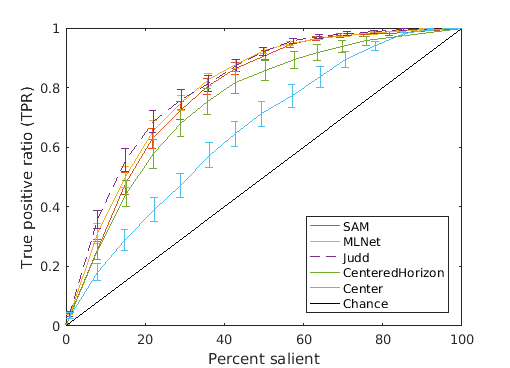
\includegraphics[width=0.7\textwidth]{images/results_fix_4_to_6_all.png} 
\end{center}
\end{frame}

\begin{frame}{Resultados fijaciones 7 a 12}
\begin{center}
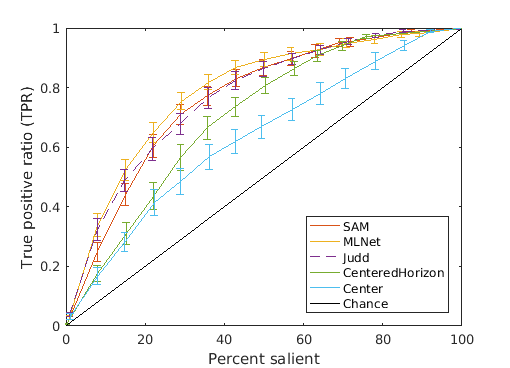
\includegraphics[width=0.7\textwidth]{images/results_fix_7_to_12_all.png} 
\end{center}
\end{frame}

\begin{frame}{Predicción del centro del círculo de respuesta}
\begin{itemize}
\item Consideramos los puntos que son centro del círculo de respuesta como si fueran fijaciones.
\item Así, utilizamos el mismo modelo de Judd que acabamos de explicar, pero agregando una feature más que modele la distancia al target.
\item Esta feature ayuda a modelar el conocimiento del target. De todas formas, testearemos en todos los ensayos y luego sólo en aquellos donde el target no fue encontrado.
\end{itemize}
\end{frame}

\begin{frame}{Predicción del centro del círculo de respuesta}
{Predicción sobre todos los ensayos, comparando con todos los humanos}
\begin{center}
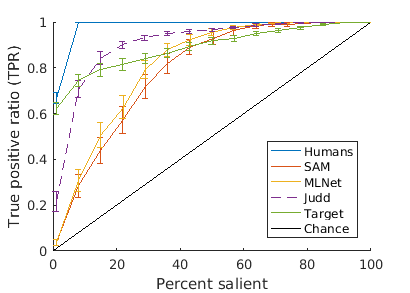
\includegraphics[width=0.7\textwidth]{images/guess_all_1.png} 
\end{center}
\end{frame}

\begin{frame}{Predicción del centro del círculo de respuesta}
{Predicción sobre los ensayos con target no encontrado, comparando con todos los humanos}

\begin{center}
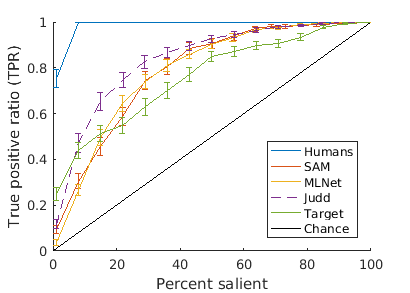
\includegraphics[width=0.7\textwidth]{images/guess_notfound_1.png} 
\end{center}
\end{frame}

\begin{frame}{Predicción del centro del círculo de respuesta}
{Predicción sobre todos los ensayos, comparando con los humanos. Para una comparación más justa, separamos los sujetos en conjunto de training y test ($\frac{3}{4}$ y $\frac{1}{4}$)}

\begin{center}
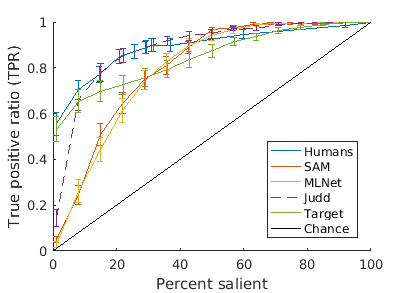
\includegraphics[width=0.7\textwidth]{images/guess_all_test_2.png} 
\end{center}
\end{frame}

\begin{frame}{Predicción del centro del círculo de respuesta}
\begin{itemize}
\item Si bien pudimos alcanzar performances muy similares a las humanas, deberíamos obtener datos de más sujetos para poder concluirlo fehacientemente.
\item Por ser un modelo de machine learning, si bien logramos predicciones muy buenas todavía no podemos describir intuitivamente cuáles son las regiones más probables.
\end{itemize}
\end{frame}

\begin{frame}{Conclusión de los modelos estáticos}

Como conclusión de todo esto vemos que pudimos superar a los modelos del estado del arte en la predicción de la tercera fijación y que logramos predecir con bastante eficiencia dónde los sujetos colocarán el centro de su círculo de respuesta.
\bigskip

El modelo estático de la tercera fijación será utilizado como base para los modelos dinámicos.
\end{frame}

\section{Modelos dinámicos}
\subsection{Modelo de Najemnik \& Geisler}
\begin{frame}{Modelos dinámicos}
Los modelos dinámicos son aquellos que no solo predicen las áreas donde
recaerán las fijaciones, sino que buscarán predecir posiciones concretas de las fijaciones y un orden probable de las mismas.

\bigskip

Para esto nos basaremos en un modelo bayesiano propuesto por Najemnik \& Geisler en 2005. 
\end{frame}

\begin{frame}{Modelo de Najemnik \& Geisler}

$$s_{i}(T) = prior(i) \cdot \prod_{t=1}^T exp\left(d'^2_{ik(t)} W_{ik(t)}\right)$$

$$p_i(T) = \displaystyle\frac{s_i(T)}{\sum_{j=1}^n s_j(T)}$$

\bigskip
$prior$ es la probabilidad a priori, $t$ es el número de fijación, $d'_{ik(t)}$ y $W_{ik(t)}$ son el mapa de visibilidad y la respuesta del target en la ubicación $i$ cuando el sujeto se encuentra fijando la vista en $k(t)$. $T$ es el número de fijación actual y $k(t)$ representa la ubicación de la fijación en tiempo $t$.

\end{frame}

\begin{frame}

\begin{figure}
\begin{center}
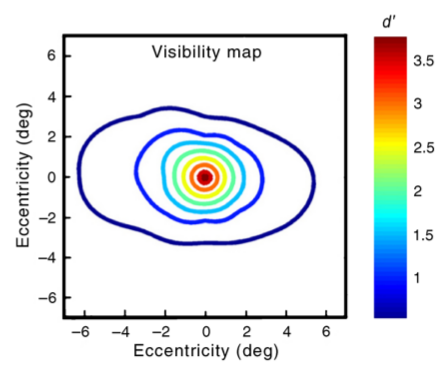
\includegraphics[width=0.5\textwidth]{images/visibility-map.png} 
\end{center}
\end{figure}

Ejemplo de mapa de visibilidad, que es lo que modela $d'$. En nuestro trabajo lo simplificamos como una gaussiana bidimensional con los parámetros de forma que imiten a los de la imagen (extraída del paper de Najemnik \& Geisler).%, pero existen otros modelos más sofisticados y computacionalmente prohibitivos para el presente trabajo, que queda como trabajo futuro. 

\end{frame}

\begin{frame}

$$k_{opt}(T+1) = \argmax\limits_{k(T+1)} \sum_{i=1}^n p_i(T)p(C|i,k(T+1))$$

donde $p(C|i,k(T+1))$ es la probabilidad de estar en lo correcto dado que la ubicación del target es $i$ y la ubicación de la próxima fijación es $k(T+1)$. $p(C|i,k(T+1))$ puede calcularse de la siguiente forma:
\end{frame}

\begin{frame}


{\footnotesize
$$p(C | i, k(T+1)) = \int\limits_{-\infty}^{+\infty}\phi(w) \prod\limits_{j \neq i} \Phi\left(\dfrac{2d'_{ik(T+1)} w -2\ln\dfrac{p_j(T)}{p_i(T)} + d_{jk(T+1)}^{\prime 2} + d_{ik(T+1)}^{\prime 2}}{2d'_{jk(T+1)}} \right) dw$$}

Optimizamos el cálculo numérico de la integral detectando un intervalo fuera del cual la integral valdrá 0 (aprovechándonos de que $\phi$ converge rápidamente a 0 lejos del 0 y que $\Phi(w)$ es menor a $10^{87}$ cuando $w < 20$).
\end{frame}

\begin{frame}{Definición de $W$}
\begin{itemize}
\item Dijimos que $W_{ik(t)}$ es la respuesta del template de la $i$-ésima posible ubicación dado que el sujeto está fijando en $k(t)$ en la fijación número $t$. 

\item En otras palabras, representa cuán parecida es la posición $i$ al target para el observador que se encuentra fijando su vista en $k(t)$. 
\item Definimos $W_{ik(t)} \in \mathcal{N}(\mu_{ik(t)}, \sigma^2_{ik(t)})$ donde:

$$ \mu_{ik(t)}
= \left\{ \begin{array}{lc}
             0.5 &  si \ i = \ ubicaci\acute{o}n \ del \ target \\
             -0.5 &  caso \ contrario 
          \end{array}
   \right.$$

$$ \sigma^2_{ik(t)} = \displaystyle\frac{1}{d'^2_{ik(t)}}$$ 
\end{itemize}
\end{frame}

\begin{frame}{Propiedades del modelo de Najemnik \& Geisler}
\begin{itemize}
\item Sin necesidad de colocarlo explícitamente, este modelo logra inhibición de retorno así como longitudes de sacadas moderadas. 
\item Una propiedad interesante del modelo es que por su naturaleza probabilística es capaz de predecir varias sucesiones de movimientos oculares según como se fije $W$.
\end{itemize}
\end{frame}

\begin{frame}{Aplicando el modelo de Geisler a nuestra tarea}
\begin{itemize}
\item El modelo de Najemnik \& Geisler fue realizado sobre una escena artificial, y a pesar de ser muy citado en la literatura nuestro trabajo es el primero que lo aplica en escenas naturales. 
\item La tarea original tenía 25 posiciones posibles a fijar, así que tuvimos que discretizar nuestra imagen con una grilla de $15 \times 20$ puntos posibles a fijar para poder computar la integral para todos los puntos en un tiempo razonable.
\item Utilizamos como $prior$ el mapa de saliencia que obtuvimos extendiendo Judd en lo que explicamos anteriormente. Además lo compararemos con la utilización de MLNet, un modelo de saliencia del estado del arte.
\end{itemize}
\end{frame}

\begin{frame}{Aplicando el modelo de Geisler a nuestra tarea (II)}
\begin{itemize}
\item Como la visibilidad tiende a cero cuando un punto está muy lejos de donde se está realizando la fijación, la varianza tendería a infinito. Es por esto que trasladamos la varianza de la siguiente forma:

$$ \sigma_{ik(t)}^1 = \displaystyle\frac{1}{a \cdot d'_{ik(t)} + b} \text{ con } a = 3 \text{ y } b = 4$$ 

Además experimentamos con otros pares $(a,b)$.
\item Además de usar $W$ como fue definido originalmente, experimentamos con una modificación 

$$\mu_{ik(t)}^2 = \mu^1_{ik(t)} \cdot \Big(d'_{ik(t)} + \dfrac{1}{2}\Big) + corr_{i} \cdot \Big(\dfrac{3}{2} - d'_{ik(t)}\Big) \in [-1, 1]$$

\end{itemize}
\end{frame}

\begin{frame}{Otros modelos dinámicos}
\begin{itemize}
\item Además de los dos modelos basados en Geisler, agregamos otros modelos baseline para comparar performance.
\item Veamos resumidamente de qué se tratan los tres modelos:
\begin{itemize}
\item Modelo de sesgo de la fijación central: toma una gaussiana bidimensional como mapa de probabilidad, con pico en el centro de la imagen
\item Modelo dinámico estadístico
\item Modelo greedy
\end{itemize}
\end{itemize}
\end{frame}

\begin{frame}[fragile]{Otros modelos dinámicos}
{Modelo dinámico estadístico}

Este modelo intenta imitar crear $scanpaths$ que imiten las características que encontramos en el análisis anterior.

\begin{center}
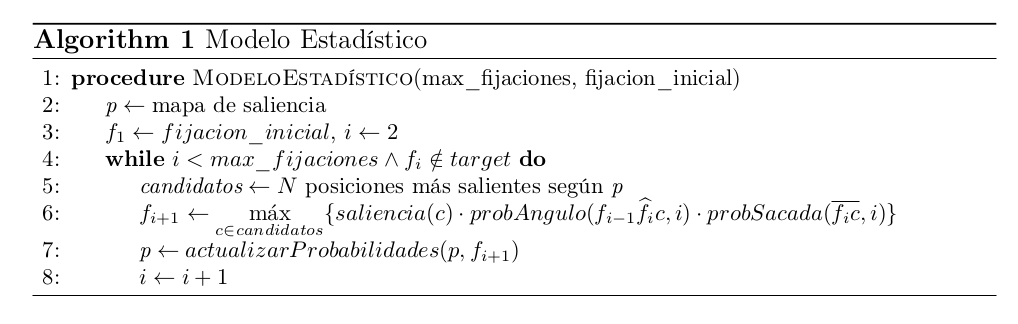
\includegraphics[width=\textwidth]{images/modelo-estadistico.png}
\end{center}

\end{frame}

\begin{frame}{Otros modelos dinámicos}
{Modelo greedy}

Este modelo toma el punto de mayor probabilidad en cada paso. Se contrapone con los modelos bayesianos, que miran una fijación hacia el futuro para decidir la fijación a realizar. 

\begin{center}
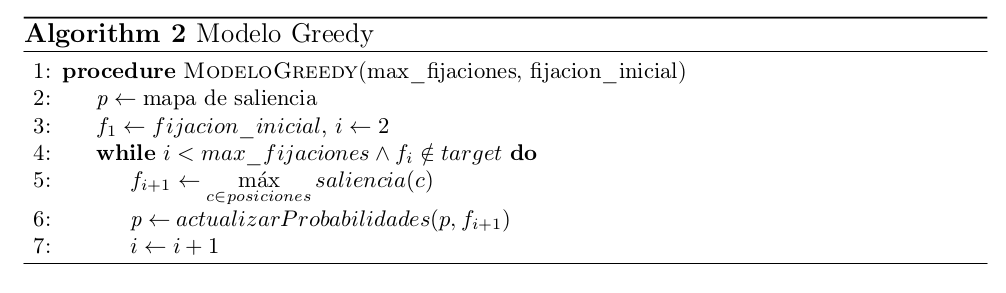
\includegraphics[width=\textwidth]{images/modelo-greedy.png}
\end{center}

\end{frame}

\begin{frame}
Vamos a analizar la performance de los cinco modelos (los tres más básicos y los dos bayesianos). Para ellos debemos definir qué métricas utilizaremos.
\end{frame}


\subsection{Métodos de comparación de scanpaths adaptados a nuestra tarea}
\begin{frame}{Métodos de comparación de scanpaths adaptados a nuestra tarea}

\begin{itemize}
\item Los métodos de comparación que mencionamos no siempre se adaptan bien a nuestra tarea, así que debimos adaptarlos.
\item Además, en los trabajos que vimos se suele hacer un análisis de consistencia entre sujetos pero no cuán parecido es un modelo predictivo a los humanos.
\end{itemize}
\end{frame}

\begin{frame}{Métricas utilizadas}
\begin{itemize}
\item Métrica de número de fijaciones esperadas para
encontrar el target, solo para ensayos exitosos.
\item Métrica de performance sobre todos los ensayos: calcula la proporción de ensayos exitosos promedio entre todos los ensayos con $c$ sacadas permitidas $c = \{2,4,8,12\}$.
\item Métrica de string edit distance.
\end{itemize}
\end{frame}

\begin{frame}{Métricas utilizadas}
{Métrica de número de fijaciones esperadas para
encontrar el target, solo para ensayos exitosos.}

Sea $s \in Sujetos$. Tomaremos todos los demás sujetos como conjunto de entrenamiento. Sea $$ E = \{(s,m) \ | \ \text{el sujeto $s$ encontró el target en la imagen $m$}\}$$

se tiene que

$$ \mu_m
= \left\{ \begin{array}{lc}
             \avg\limits_{j:(j,m) \in E} cf_{j,m} &  si \ |\{j:(j,m) \in E\}| \geq 3 \\
             +\infty &  \text{caso contrario}
          \end{array}
   \right.$$

$$mean\_length_s = \avg\limits_{m:(s,m) \in E} |cf_{s,m} - \mu_m| $$

$mean\_length_s$ es el valor que tomaremos como métrica.
\end{frame}

\begin{frame}{Métricas utilizadas}
{Métrica de string editing distance}

Sea $s \in Sujetos$. Calcularemos la edit distance media por imagen de todos los scanpaths de longitud al menos $c$, truncando solo las primeras $c$ fijaciones ($c \in \{2,4,6,8,10\}$). Sea $\mu_{m,c}^{lev}$ a la string edit distance media de la imagen $m$ en la categoría $c$.

$$\mu_{m,c,s}^{lev} = \avg\limits_{s \neq i} \ lev(scanpath_{s,m}[1..c], scanpath_{i,m}[1..c])$$

$$mean\_lev_{s,c} = \avg\limits_{1 \leq m \leq |images|} \ |\mu_{m,c}^{lev} - \mu_{m,c,s}^{lev}|$$

$mean\_lev_{s,c}$ es el valor que tomaremos como métrica.
\end{frame}

\begin{frame}
\begin{itemize}
\item Repetimos el procedimiento separando cada vez un sujeto $s$ diferente.
\item Luego, cuando queremos comparar un nuevo modelo contra los humanos, tomamos a $s$ como el nuevo modelo y todos los humanos irán al conjunto de entrenamiento.
\item ¿Cómo cuantificamos cuán parecido es un modelo a los sujetos?
\end{itemize}
\end{frame}


\begin{frame}
\begin{itemize}
\item Aplicamos tres tests de normalidad para todas las métricas en todas sus categorías.
\item Los tests de normalidad son tests de hipótesis cuya hipótesis nula es que la muestra pertenece a una distribución normal.
\item En la gran mayoría de los casos no pudo rechazarse la hipótesis nula, por lo que podemos decir que los datos no están fuertemente sesgados.
\end{itemize}
\end{frame}

\begin{frame}
\begin{itemize}
\item Como los datos no están fuertemente sesgados, calcularemos la media y la varianza y veremos cuán similar es un valor al resto de la muestra utilizando el \textit{z-score}.
\item El \textit{z-score} o \textit{Standard score} se define como

$$ z = \left| \dfrac{x-\mu}{\sigma}\right|$$

es decir, cuán lejos se encuentra $x$ de la media en unidades de desvío estándar.
\end{itemize}
\end{frame}

\subsection{Resultados de modelos dinámicos}
\begin{frame}{Resultados respecto de la primera métrica}
{Métrica de número de fijaciones esperadas para
encontrar el target, solo para ensayos exitosos $z_{length}^s$.}

\begin{center}
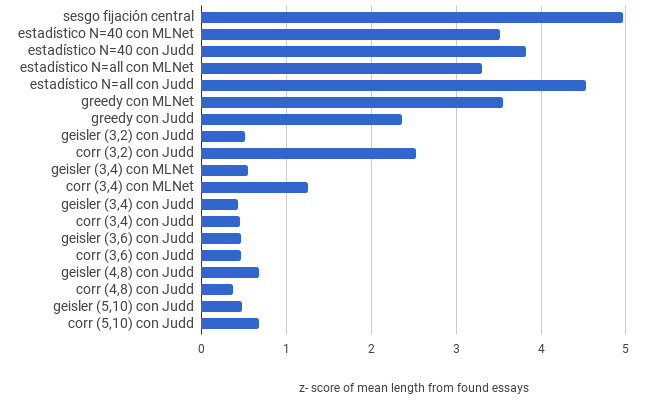
\includegraphics[width=0.7\textwidth]{images/z-score-mean-length.png}
\end{center}

{\scriptsize Logramos separar bien los modelos menos complejos de los bayesianos. Recordemos que como utilizamos \textit{z-score}, \textbf{cuanto menor el valor obtenido, mejor}.}
%/home/melanie/Downloads/tesis-de-licenciatura/results/z-score-mean-length.png
%/home/melanie/Downloads/tesis-de-licenciatura/results/z-score-percent-found.png
\end{frame}

\begin{frame}{Resultados respecto de la segunda métrica}
{Métrica de performance sobre todos los ensayos: calcula la proporción de ensayos exitosos promedio entre todos los ensayos con $c$ sacadas permitidas $c = \{2,4,8,12\}$}

\begin{center}
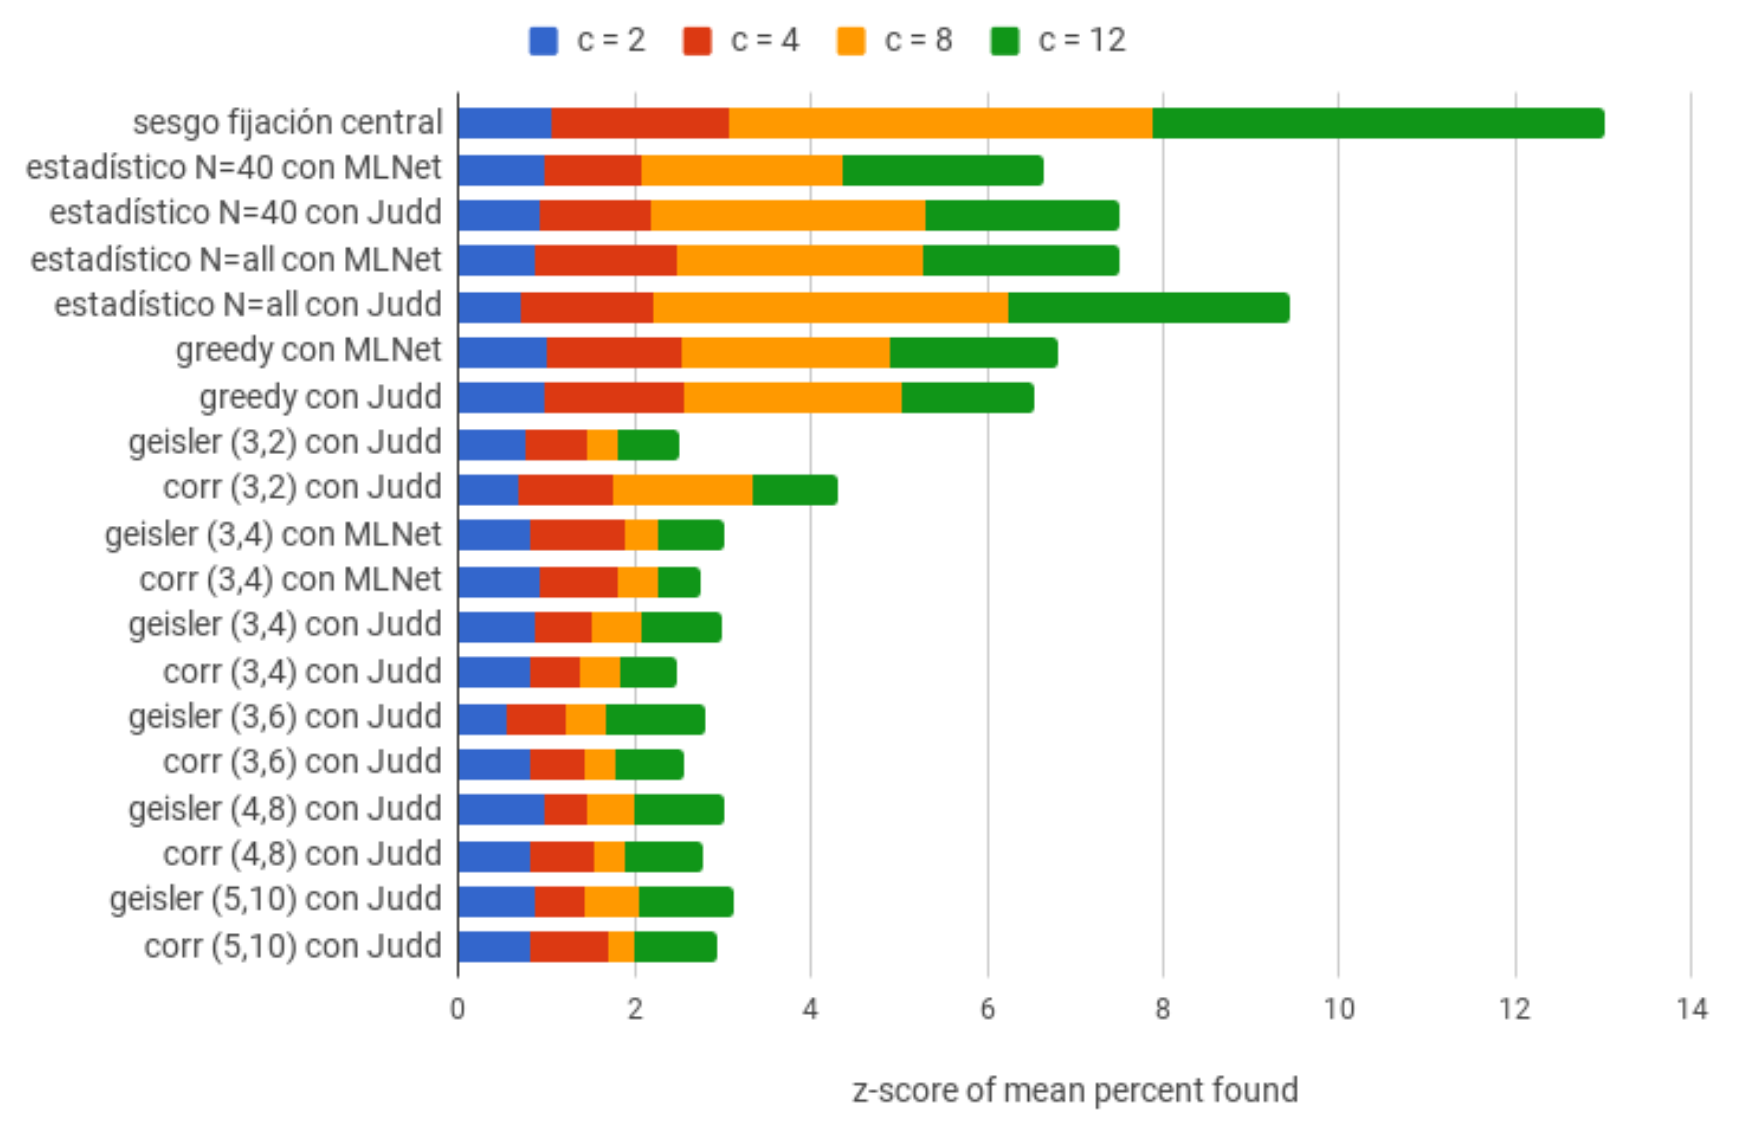
\includegraphics[width=0.9\textwidth]{images/z-score-percent-found.png}
\end{center}

\end{frame}

\begin{frame}{Resultados respecto de la segunda métrica}
{Métrica de performance sobre todos los ensayos: calcula la proporción de ensayos exitosos promedio entre todos los ensayos con $c$ sacadas permitidas $c = \{2,4,8,12\}$}

Nuevamente, la segunda métrica logró separar los modelos de los bayesianos de los otros, con una clara ventaja de los modelos bayesianos. Como nuestra métrica tiene 4 categorías, sumamos los \textit{z-score} de las 4 categorías para el análisis.
\end{frame}

\begin{frame}{Resultados respecto de la tercera métrica}
{Métrica de string edit distance}

\begin{center}
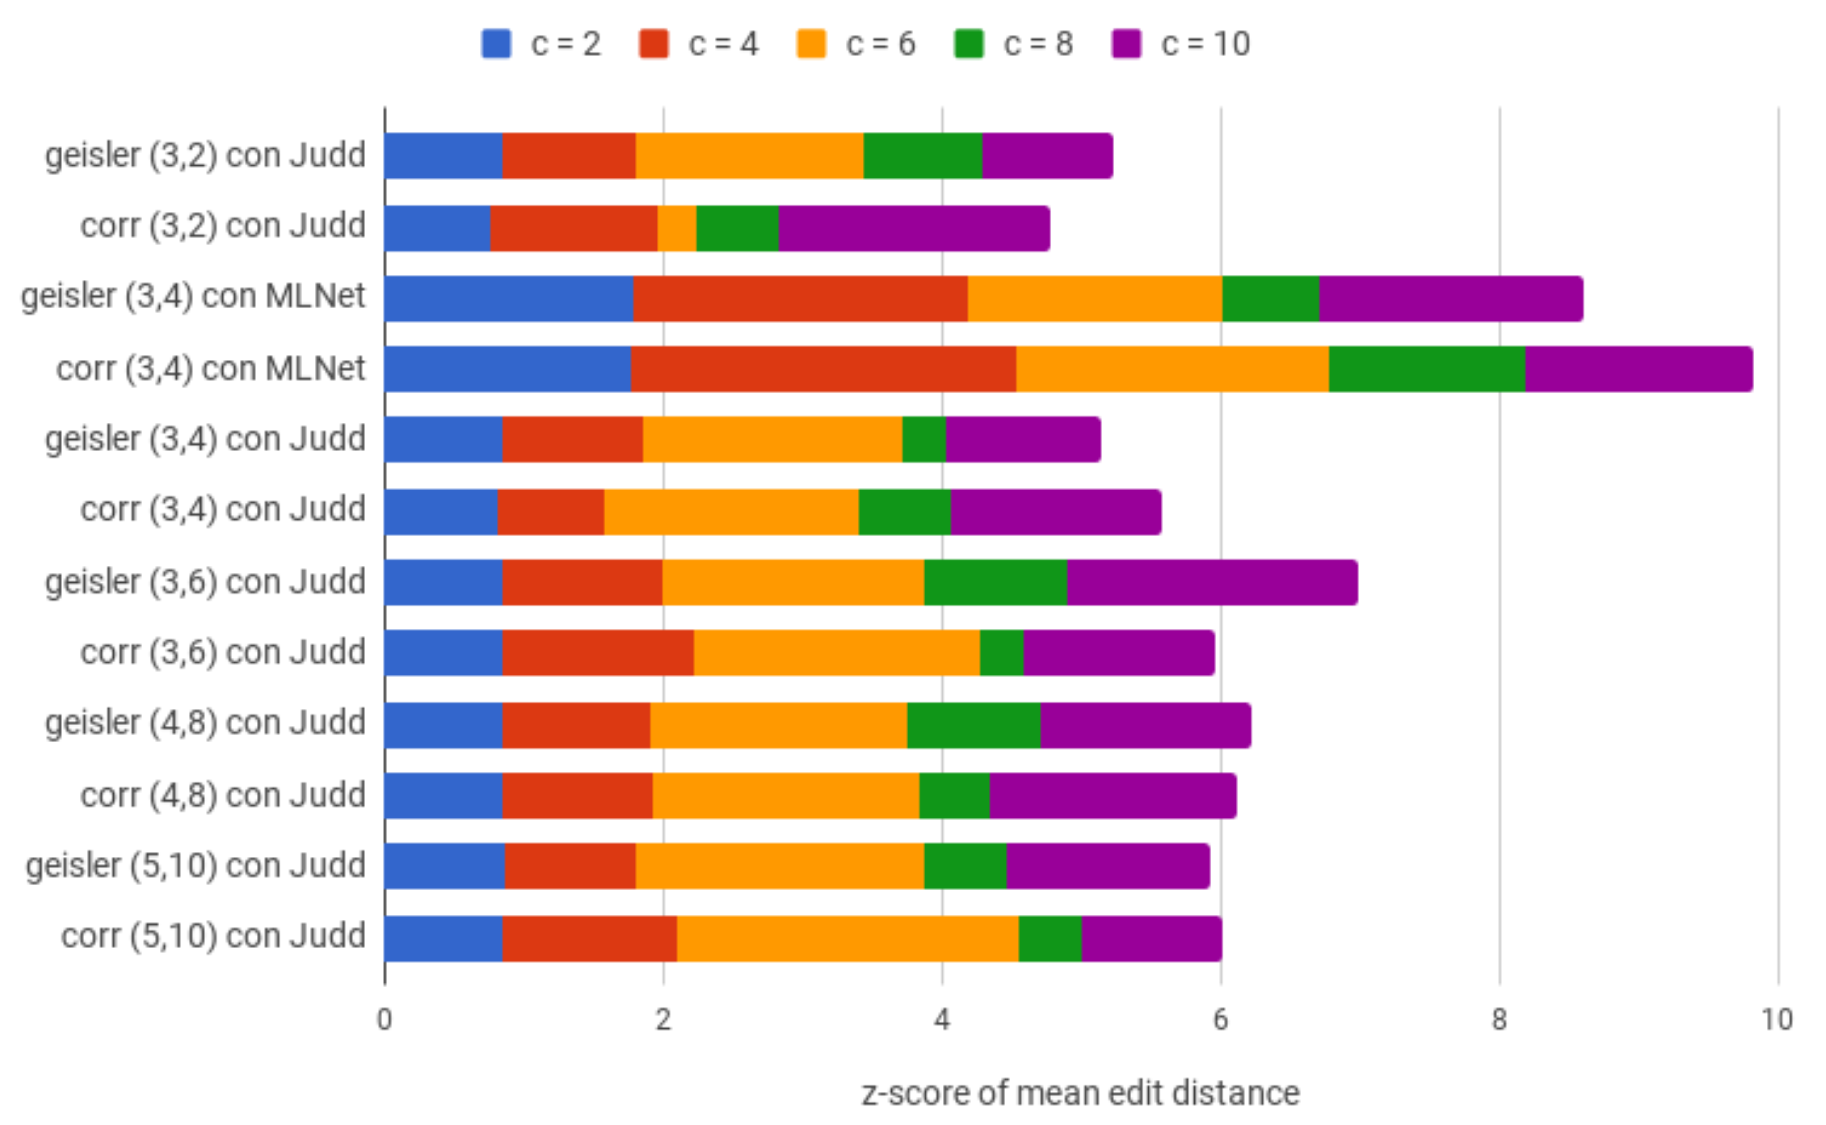
\includegraphics[width=\textwidth]{images/z-score-mean-edit-distance.png}
\end{center}

\end{frame}

\begin{frame}{Resultados respecto de la tercera métrica}
{Métrica de string edit distance}
\begin{itemize}
\item La performance de los modelos es muy similar para aquellos con baja variabilidad, es decir, para pares $(a, b)$ más altos. \item La performance parece mejorar levemente para modelos de más alta varianza. Esto puede producirse porque al bajar la variabilidad el modelo simula un poco peor la existencia
de distractores y equivocaciones en el juzgamiento de la mejor posición para obtener el target.
\item \textbf{Se observa una mejora utilizando nuestro modelo de saliencia como base respecto de MLNet.}
\end{itemize}
\end{frame}

\begin{frame}{Conclusiones de los modelos dinámicos}
\begin{itemize}
\item El modelo $greedy$ obtuvo una performance mucho peor que los modelos bayesianos, por lo que concluimos que considerar una fijación hacia el futuro logra modelar una búsqueda visual más similar a la humana
\item Los modelos no bayesianos tuvieron performance muy pobres
\item El modelo de Geisler original con constantes $(3,2)$ o $(3,4)$ o el modelo de Geisler modificado con constantes $(3,4)$ parecen buenas elecciones.
\item Se observa una mejora utilizando nuestro modelo de saliencia como base (Judd extendido) respecto de MLNet.
\end{itemize}
\end{frame}

\section{Conclusiones}
\begin{frame}{Conclusiones generales}
\begin{itemize}
\item Creamos un corpus de imágenes y de descripción de objetos que abrimos a la comunidad.
\item Creamos un modelo de saliencia que predice mejor la tercera fijación que los modelos del estado del arte. ¡Aún hay muchos puntos para mejorar aún más!
\item Predijimos con muy buenos resultados los centros de los círculos de respuesta y describimos ciertas características de los radios de los círculos de respuesta.
\item Reprodujimos por primera vez el modelo de Geisler en escenas naturales, con resultados muy prometedores.
\end{itemize}
\end{frame}

\begin{frame}{Trabajos futuros}
\begin{itemize}
\item Amplificar el corpues de imágenes y de descripción de objetos para confirmar más fuertemente los resultados.
\item Explorar distintos aspectos de los features tipo II para extraer más datos. Este approach es novedoso con respecto a los otros trabajos que vimos.
\item Utilizar un mapa de visibilidad más sofisticado, por ejemplo el de Bradley et al. 2004.
\item Reprodujimos por primera vez el modelo de Geisler en escenas naturales, con resultados muy prometedores.
\end{itemize}
\end{frame}


\begin{frame}
\begin{center}
\Huge ¡Gracias!

\bigskip

\huge ¿Preguntas?
\end{center}
\end{frame}

\end{document}
